\section{Methodology}
\label{sec:Methodology}

In this section, we present the details of the Evidence-Enhanced Large Vision-Language Model (E2LVLM). The proposed E2LVLM endeavors to utilize textual evidence related to authentic images for debunking multimodal OOC misinformation. The framework is illustrated in \Cref{fig:2}.

%---------------------------------------
\begin{figure*}
  \centering
      \includegraphics[width=\linewidth]{fig3.jpg}
    \caption{Prompts and their examples in E2LVLM. (a) Reranking prompt $\mathcal{P}_\mathrm{rerank}$ is to select one most relevant textual evidence related to the authentic image. (b) Rewriting prompt $\mathcal{P}_\mathrm{rewrite}$ is to achieve the coherent and contextually attuned content for alignment. (c) Explanation prompt $\mathcal{P}_\mathrm{Expla.}$ is to generate the compelling rationale to make up support for its assessment. (d) Tuning prompt $\mathcal{P}_\mathrm{OOC}$ is to extend the general-purpose LVLM to the task of multimodal out-of-context misinformation detection.}
    \label{fig:3}
\end{figure*}

\subsection{Task Definition and Background}

Given an authentic image $v$ and its claim $t$ from a dataset $\mathcal{D}$, where the image-claim pair $(v,t)\in\mathcal{D}$ achieves a multitude of evidence $(v_e, t_e)$ gathered by~\cite{abdelnabi2022open}, the task of OOC misinformation detection is to acquire a model $f_{ooc}(v,t,v_e, t_e)$ that makes a prediction $\hat{y}$ regarding the authenticity of the image-claim pair. Each pair is assigned with a semantic label $y\in\{0,1\}$, being either the ``Falsified'' (out-of-context) $(1)$ or ``Pristine'' (not out-of-context) $(0)$.

A typical approach to this issue is to train a classifier that provides a probability $p_{ooc}=p(\hat{y}|v,t,v_e, t_e)$. A more attractive solution taken by Qi \etal~\cite{qi2024sniffer} is to fine-tune the general-domain LVLM $g(v,t,v_e, t_e;\theta)$ on this task-specific dataset, thereby yielding the token $\mu$ of the corresponding semantic label. The symbol $\theta$ represents the learnable parameters of the LVLM model during training.

In the context of LVLMs, existing methods for discerning multimodal OOC misinformation typically default to the use of all the evidence $v_e$, $t_e$ of the image $v$ and claim $t$, but for image-evidence, the long distance between them inevitably prevents the model's discriminatory powers in the sense. Upon investigating the realm of OOC, we summarize the following findings:

\begin{enumerate}[label=\arabic*.]
    \item The fine-tuning model should not require access to all the evidence regarding image-claim pairs.
    \item The LVLMs-based model should require coherent and contextually attuned content, rather than pieces of external information.
    \item Similarly, the model should require both judgment and explanation, because this supervised signal contributes to the model's discriminatory powers.
\end{enumerate}

\subsection{Textual Evidence Reranking and Rewriting}

To rerank the gathered textual evidence of authentic images for acquiring relevant items, the most intuitive solution is to directly depend on the cosine similarity to calculate the relevance between the image $v$ and textual evidence $v_e=\{v^1_e, v^2_e,...,v^k_e\}$, \ie, $\mathrm{argsort}\ sim(\mathbf{z}_v, \mathbf{z}_{v^k_e})$, where $sim(\cdot)$ represents the cosine similarity, $\mathbf{z}_v\in\mathbb{R}^{1\times dim}$ and $\mathbf{z}_{v^k_e}\in\mathbb{R}^{1\times dim}$ denote the $dim$-dimensionality representations of the image and $k$-th evidence, respectively. However, this solution seriously lies in representation quality extracted by chosen backbone encoders (\eg, ViT B/32~\cite{radford2021learning} and ViT L/14~\cite{li2023blip}), and suffers from complex context. This is a sub-optimal option. To overcome this issue, we tend to multimodal understanding and reranking capabilities of LVLMs, and devise a textual evidence reranking strategy.

Textual evidence reranking refers to adopting the LVLM model Qwen2-VL~\cite{wang2024qwen2} to select one most relevant textual evidence $v^r_e$ related to the image. Due to the length extrapolation capability of Qwen2-VL, we incorporate the authentic image and its retrieved textual evidence as the part of the reranking prompt, denoted as $\mathcal{P}_\mathrm{rerank}(v, v_e)$. To finely control the output format, we attach a simple yet effective demonstration to the corresponding prompt. We present this prompt and its example in subfigure (a) of \Cref{fig:3}.

Further, in order to alleviate the discrepancy between the selected textual evidence $v^r_e$ and natural language-based LVLMs for alignment, we design a textual evidence rewriting strategy. Similar to the input prompt of the LVLM model for rerank, we leverage $(v, v^r_e)$ as part of the rewriting prompt, denoted as $\mathcal{P}_\mathrm{rewrite}(v, v^r_e)$, to guide the model for generating coherent and attuned content $\widetilde{v}^r_e$. Such prompt and its example are depicted in subfigure (b) of \Cref{fig:3}.

Additionally, we observe the fact that access to textual evidence of images is not invariably retrieved by search engines. In response to the lack of such textual evidence in the OOC realm, we directly employ the LVLM model to produce image captions as the rewritten content $\widetilde{v}^r_e$.
% \documentclass{standalone}
%\usetikzlibrary{...}
\usepackage{tikz}
\begin{document}
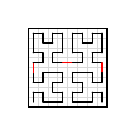
\begin{tikzpicture}
\tikzstyle{helperline} = [lightgray!60!white, line width=0.1mm];
\draw[line cap=round][helperline] (-0.0,0.125) -- (1.0,0.125);
\draw[line cap=round][helperline] (-0.0,0.25) -- (1.0,0.25);
\draw[line cap=round][helperline] (-0.0,0.375) -- (1.0,0.375);
\draw[line cap=round][helperline] (-0.0,0.5) -- (1.0,0.5);
\draw[line cap=round][helperline] (-0.0,0.625) -- (1.0,0.625);
\draw[line cap=round][helperline] (-0.0,0.75) -- (1.0,0.75);
\draw[line cap=round][helperline] (-0.0,0.875) -- (1.0,0.875);
\draw[line cap=round][helperline]  (0.125,1.0) -- (0.125,-0.0);
\draw[line cap=round][helperline]  (0.25,1.0) -- (0.25,-0.0);
\draw[line cap=round][helperline]  (0.375,1.0) -- (0.375,-0.0);
\draw[line cap=round][helperline]  (0.5,1.0) -- (0.5,-0.0);
\draw[line cap=round][helperline]  (0.625,1.0) -- (0.625,-0.0);
\draw[line cap=round][helperline]  (0.75,1.0) -- (0.75,-0.0);
\draw[line cap=round][helperline]  (0.875,1.0) -- (0.875,-0.0);
\draw[line cap=round]  (0,1) rectangle (1,0);
\draw[line cap=round] (0.0625, 0.0625) -- (0.0625, 0.1875);
\draw[line cap=round] (0.0625, 0.1875) -- (0.1875, 0.1875);
\draw[line cap=round] (0.1875, 0.1875) -- (0.1875, 0.0625);
\draw[line cap=round] (0.1875, 0.0625) -- (0.3125, 0.0625);
\draw[line cap=round] (0.3125, 0.0625) -- (0.4375, 0.0625);
\draw[line cap=round] (0.4375, 0.0625) -- (0.4375, 0.1875);
\draw[line cap=round] (0.4375, 0.1875) -- (0.3125, 0.1875);
\draw[line cap=round] (0.3125, 0.1875) -- (0.3125, 0.3125);
\draw[line cap=round] (0.3125, 0.3125) -- (0.4375, 0.3125);
\draw[line cap=round] (0.4375, 0.3125) -- (0.4375, 0.4375);
\draw[line cap=round] (0.4375, 0.4375) -- (0.3125, 0.4375);
\draw[line cap=round] (0.3125, 0.4375) -- (0.1875, 0.4375);
\draw[line cap=round] (0.1875, 0.4375) -- (0.1875, 0.3125);
\draw[line cap=round] (0.1875, 0.3125) -- (0.0625, 0.3125);
\draw[line cap=round] (0.0625, 0.3125) -- (0.0625, 0.4375);
\draw[line cap=round,red] (0.0625, 0.4375) -- (0.0625, 0.5625);
\draw[line cap=round] (0.0625, 0.5625) -- (0.1875, 0.5625);
\draw[line cap=round] (0.1875, 0.5625) -- (0.1875, 0.6875);
\draw[line cap=round] (0.1875, 0.6875) -- (0.0625, 0.6875);
\draw[line cap=round] (0.0625, 0.6875) -- (0.0625, 0.8125);
\draw[line cap=round] (0.0625, 0.8125) -- (0.0625, 0.9375);
\draw[line cap=round] (0.0625, 0.9375) -- (0.1875, 0.9375);
\draw[line cap=round] (0.1875, 0.9375) -- (0.1875, 0.8125);
\draw[line cap=round] (0.1875, 0.8125) -- (0.3125, 0.8125);
\draw[line cap=round] (0.3125, 0.8125) -- (0.3125, 0.9375);
\draw[line cap=round] (0.3125, 0.9375) -- (0.4375, 0.9375);
\draw[line cap=round] (0.4375, 0.9375) -- (0.4375, 0.8125);
\draw[line cap=round] (0.4375, 0.8125) -- (0.4375, 0.6875);
\draw[line cap=round] (0.4375, 0.6875) -- (0.3125, 0.6875);
\draw[line cap=round] (0.3125, 0.6875) -- (0.3125, 0.5625);
\draw[line cap=round] (0.3125, 0.5625) -- (0.4375, 0.5625);
\draw[line cap=round,red] (0.4375, 0.5625) -- (0.5625, 0.5625);
\draw[line cap=round] (0.5625, 0.5625) -- (0.6875, 0.5625);
\draw[line cap=round] (0.6875, 0.5625) -- (0.6875, 0.6875);
\draw[line cap=round] (0.6875, 0.6875) -- (0.5625, 0.6875);
\draw[line cap=round] (0.5625, 0.6875) -- (0.5625, 0.8125);
\draw[line cap=round] (0.5625, 0.8125) -- (0.5625, 0.9375);
\draw[line cap=round] (0.5625, 0.9375) -- (0.6875, 0.9375);
\draw[line cap=round] (0.6875, 0.9375) -- (0.6875, 0.8125);
\draw[line cap=round] (0.6875, 0.8125) -- (0.8125, 0.8125);
\draw[line cap=round] (0.8125, 0.8125) -- (0.8125, 0.9375);
\draw[line cap=round] (0.8125, 0.9375) -- (0.9375, 0.9375);
\draw[line cap=round] (0.9375, 0.9375) -- (0.9375, 0.8125);
\draw[line cap=round] (0.9375, 0.8125) -- (0.9375, 0.6875);
\draw[line cap=round] (0.9375, 0.6875) -- (0.8125, 0.6875);
\draw[line cap=round] (0.8125, 0.6875) -- (0.8125, 0.5625);
\draw[line cap=round] (0.8125, 0.5625) -- (0.9375, 0.5625);
\draw[line cap=round,red] (0.9375, 0.5625) -- (0.9375, 0.4375);
\draw[line cap=round] (0.9375, 0.4375) -- (0.9375, 0.3125);
\draw[line cap=round] (0.9375, 0.3125) -- (0.8125, 0.3125);
\draw[line cap=round] (0.8125, 0.3125) -- (0.8125, 0.4375);
\draw[line cap=round] (0.8125, 0.4375) -- (0.6875, 0.4375);
\draw[line cap=round] (0.6875, 0.4375) -- (0.5625, 0.4375);
\draw[line cap=round] (0.5625, 0.4375) -- (0.5625, 0.3125);
\draw[line cap=round] (0.5625, 0.3125) -- (0.6875, 0.3125);
\draw[line cap=round] (0.6875, 0.3125) -- (0.6875, 0.1875);
\draw[line cap=round] (0.6875, 0.1875) -- (0.5625, 0.1875);
\draw[line cap=round] (0.5625, 0.1875) -- (0.5625, 0.0625);
\draw[line cap=round] (0.5625, 0.0625) -- (0.6875, 0.0625);
\draw[line cap=round] (0.6875, 0.0625) -- (0.8125, 0.0625);
\draw[line cap=round] (0.8125, 0.0625) -- (0.8125, 0.1875);
\draw[line cap=round] (0.8125, 0.1875) -- (0.9375, 0.1875);
\draw[line cap=round] (0.9375, 0.1875) -- (0.9375, 0.0625);
\end{tikzpicture}
\end{document}

\subsection{OOC Multimodal Instruction Dataset}

For the news domain and OOC detection task, a multimodal instruction dataset with both judgment and explanation is constructed to enhance the model's discriminatory powers. Although the previous method~\cite{qi2024sniffer} adopts InstructBLIP~\cite{dai2023instructblip} converting images into textual descriptions (as if it could visualize the image) and uses the close-source language-only GPT-4~\cite{achiam2023gpt} to capture inconsistencies between them, this destroys informative content related to authentic images. We summarize this issue stemming from a cross-modal semantic gap between images and the corresponding textual descriptions~\cite{jiang2024hallucination}. Therefore, we retain authentic images for claims in the OOC detection.

By leveraging Qwen2-VL~\cite{wang2024qwen2}, we adjust the model to follow an explanation prompt $\mathcal{P}_{Expla.}$, as shown in subfigure (c) of \Cref{fig:3}. Typically, we provide $(v,t, \widetilde{v}^r_e)$ as the part of this prompt that queries Qwen2-VL~\cite{wang2024qwen2} to perform desired behaviors, \ie, generating compelling explanations to support their judgments for the falsified information. The whole process can be defined as follows,
\begin{equation}\label{eq:vcg_5}
  \widetilde{\mathcal{D}} = \{(x,\widetilde{v}^r_e,{t}^r_e),s\mid x \sim \mathcal{D}, s \sim g(s \mid I(v,t,\widetilde{v}^r_e))\},
\end{equation}
where $I(v,t,\widetilde{v}^r_e)$ denotes an instantiated instruction by presenting an image-claim pair $(v,t)$ and the rewritten content $\widetilde{v}^r_e$. Besides, $g$ and $s$ refer to the LVLM model and its output, respectively. The sign $x$ is the sample $(v,t)$, and ${t}^r_e$ denotes the most relevant item related to the claim $t$. This item is achieved by cosine similarity, unless otherwise specified. As for NewsCLIPpings~\cite{luo2021newsclippings}, the constructed OOC multimodal instruction dataset $\widetilde{\mathcal{D}}$ consists of instructions with an equal number of falsified samples and pristine samples.
\subsection{Evidence-enhanced Fine-tuning}

Regarding the identified challenge in the LVLM model Qwen2-VL~\cite{wang2024qwen2} when it comes to the OOC detection task, we suggest a one-stage multimodal instruction tuning solution extending the general-purpose LVLM, to the news domain for discerning multimodal OOC misinformation.

Our evidence-enhanced fine-tuning strategy is to provide both judgments and explanations for each image-claim pair. Simply put, we introduce both questions and candidate answers~\cite{shao2023prompting} into the tuning prompt $\mathcal{P}_\mathrm{OOC}(v,t,\widetilde{v}^r_e,{t}^r_e)$ that serves as informative inputs of the model. This makes the LVLM model unleash the potential knowledge behind itself~\cite{liu2024fka}, which explicitly analyzes the discrepancy between candidate answers for more accurate decisions. An illustration of the model response is shown in subfigure (d) of \Cref{fig:3}. For an image-claim pair with the ``Falsified'' label, we utilize the image $v$, claim $t$, rewritten textual evidence $\widetilde{v}^r_e$, and reranked visual evidence ${t}^r_e$ to format the input prompt of the LVLM model for response generation. The model provides the response likewise ``$<$Judgment$>$ $<$Explanation$>$'', where $<$Judgment$>$ indicates the symbol (\ie, ``No'') associated with candidate answers, and $<$Explanation$>$ is a coherent sentence serving as the compelling rationale for supporting its assessment.

In order to align the initial training way of the LVLM model, we employ LoRA technology~\cite{hu2022lora} and the next token prediction loss for assessing the model’s output error. Therefore, the learning objective of the proposed model E2LVLM over the OOC task, which can be described as,
\begin{equation}\label{eq:vcg_5}
    \mathcal{L}_{\mathrm{ooc}} = \sum_{i=1}^{N} -\log P(\epsilon_i \mid v_i,t_i,\widetilde{v_i}^r_e, {t_i}^r_e, \theta_{\mathrm{ooc}}),
\end{equation}
where, $\epsilon_i$ is considered as the generated tokens of both judgment and explanation corresponding to the formatted input $(v_i,t_i,\widetilde{v_i}^r_e,{t_i}^r_e)$, and $\theta_{\mathrm{ooc}}$ refers to the learnable parameters of E2LVLM during training. Besides, $N$ is the size of $\widetilde{\mathcal{D}}$.